\RequirePackage[l2tabu, orthodox]{nag}
\documentclass[a4paper,parskip=half]{scrartcl}
\usepackage[english]{babel}
\usepackage[T1]{fontenc}
\usepackage[utf8]{inputenc}
\usepackage[pdftex]{graphicx}
\usepackage{mdwlist}
\usepackage{array}
\usepackage{multirow}
\usepackage{textcomp}
\usepackage{float}
\usepackage{xspace}
\usepackage{rotating}
\usepackage{placeins}
\usepackage{bytefield}
\usepackage[pdftex,dvipsnames,table,xcdraw]{xcolor}  % Coloured text etc.
\usepackage[activate={true,nocompatibility},stretch=10,shrink=10,factor=1100,babel=true]{microtype}

\usepackage{tikz}
\usepackage{tikz-qtree}
\usetikzlibrary{babel,arrows,positioning,calc,fit}

\PassOptionsToPackage{hyphens}{url}\usepackage[hidelinks]{hyperref}
\usepackage[compatibility=false]{caption}
\usepackage{subcaption}

\usepackage{minted}
\usemintedstyle{autumn}
% \usemintedstyle{bw} % use for black and white
\newminted{java}{gobble=1,linenos,numberblanklines=false,frame=lines,tabsize=4}
\newminted{c}{gobble=1,linenos,numberblanklines=false,frame=lines,tabsize=4}
\newminted{xml}{frame=none,tabsize=1,fontsize=\small}
\newminted{cpp}{frame=lines,tabsize=4}

\usepackage{xpatch,letltxmacro}
\LetLtxMacro{\cminted}{\minted}
\let\endcminted\endminted
\xpretocmd{\cminted}{\RecustomVerbatimEnvironment{Verbatim}{BVerbatim}{}}{}{}

\usepackage[nameinlink]{cleveref}

\newcommand{\bitlabel}[2]{%
\bitbox[]{#1}{%
\raisebox{0pt}[4ex][0pt]{%
\turnbox{45}{\fontsize{7}{7}\selectfont#2}%
}%
}%
}

\newcommand{\colorbitbox}[4]{%
\rlap{\bitbox[]{#2}{\color{#1}\rule{\width}{\height}}}%
\bitbox[#4]{#2}{#3}}

\definecolor{mygreen}{HTML}{097054}
\definecolor{myyellow}{HTML}{FFDE00}
\definecolor{myblue}{HTML}{6599FF}
\definecolor{myorange}{HTML}{FF9900}

\newcommand{\nocontentsline}[3]{}%
\newcommand{\tocless}[2]{\bgroup\let\addcontentsline=\nocontentsline#1{#2}\egroup}%

% Abbreviations
\newcommand{\java}{{\small Java}\xspace}
\newcommand{\python}{{\small Python}\xspace}
\newcommand{\cpp}{{\small C++}\xspace}
\newcommand{\xmlmate}{\textsc{XMLmate}\xspace}
\newcommand{\evosuite}{\textsc{EvoSuite}\xspace}
\newcommand{\xml}{{\small XML}\xspace}
\newcommand{\xsd}{{\small XML Schema Definition}\xspace}
\newcommand{\xom}{{\small XOM}\xspace}
\newcommand{\pin}{{\small Pin}\xspace}
\newcommand{\pcap}{{\small pcap}\xspace}
\newcommand{\png}{{\small png}\xspace}
\newcommand{\zmq}{{\small ØMQ}\xspace}
\newcommand{\msgpack}{{\small MessagePack}\xspace}
\newcommand{\xerces}{{\small Xerces2}\xspace}
\newcommand{\libpng}{\texttt{libpng}\xspace}
\newcommand{\libpcap}{\texttt{libpcap}\xspace}
\newcommand{\libxml}{\texttt{libxml2}\xspace}


\begin{document}
\pagenumbering{roman} %
\begin{titlepage}
\begin{center}
{\LARGE \bfseries Saarland University \\
Faculty of Natural Sciences and Technology I \\[0.1cm]
Department of Computer Science}\\[2.5cm]

{\Large \bfseries Master's Thesis}\\[1cm]
\unsure{Confirm title}
{\LARGE \bfseries Adapting XMLMate to Binary Subjects}\\[2cm]
{\small \bfseries submitted by}\\[0.5cm]
{\large \bfseries Nikolas Havrikov}\\[1cm]
{\small \bfseries submitted on}\\
\change {update date}
20.03.2015\\[2.5cm]
{\bfseries Supervisor}\\[0.2cm]
Prof. Andreas Zeller\\[1cm]
{\bfseries Advisor}\\[0.2cm]
\unsure{verify advisor}
Matthias Höschele\\[1cm]
{\bfseries Reviewers}\\[0.2cm]
Prof. Andreas Zeller\\[.2cm]
Dr. Christian Rossow
\end{center}
\end{titlepage}
\newpage
\begin{center}
{\LARGE \bfseries Eidesstattliche Erklärung}\\[0.2cm]
Ich erkläre hiermit an Eides Statt, 
dass ich die vorliegende Arbeit selbstständig verfasst und keine anderen als die angegebenen Quellen 
und Hilfsmittel verwendet habe.\\[1cm]
{\LARGE \bfseries Statement in Lieu of an Oath}\\[0.2cm]
I confirm under oath that I have written this thesis on my own and that I 
have not used any other media or materials than the ones referred to in this thesis.\\[3cm]
{\LARGE \bfseries Einverständniserklärung}\\[0.2cm]
Ich bin damit einverstanden, dass meine (bestandene) Arbeit in beiden Versionen in die 
Bibliothek der Informatik aufgenommen und damit veröffentlicht wird.\\[1cm]
{\LARGE \bfseries Declaration of Consent}\\[0.2cm]
I agree to make both versions of my thesis (with a passing grade) accessible to the public 
by having them added to the library of the Computer Science Department.\\[3cm]
\end{center}
\vfill
\begin{flushleft}
\begin{tabular}{ll@{\hspace{4.2cm}}r}
    Saarbrücken, & \rule[-2pt]{2.9cm}{.4pt} & \rule[-2pt]{4.4cm}{.4pt} \\[0px]
     & (Datum / Date) & (Unterschrift / Signature) \\
\end{tabular}
\end{flushleft}
\newpage
\section*{Acknowledgements}
This thesis has benefited from the support of several people, whom I would like to thank sincerely.
I would especially like to thank
\begin{description*}
	\item[] Andreas Zeller
	\item[] Christian Rossow
	\item[] Giorgi Maisuradze
	\item[] Matthias Höschele
	\item[] Juan Pablo Galeotti
	\item[] 
\end{description*}
\change[inline]{flesh out acknowledgements}
\newpage
\section*{Abstract}
%%%Motivation - want find vulns when autotesting
When generating test inputs with the goal of revealing failures and vulnerabilities in a program, 
%%%Problem - inputs must be well-formed
the inputs must adhere to a format specific to this program, otherwise they are 
quickly discarded without getting anywhere near executing importnat code responsible for program logic.
%%%Methodology - grammars + search-based + specific criteria
Several techniques can be used to profitably apply automated test input generation in this usage scenario -
they include leveraging format description grammars, employing search-based instance development algorithms,
and utilizing guidance criteria specifically designed for individual vulnerability classes.
%%%Results - prototype, subjects, failures
A prototypical implementation extending the search-based input generator \emph{XMLMate} with the suggested
techniques has been applied to several file formats and their corresponding libraries and has shown promise as
it detected defects, some of which are classified as security threats in the database of common
vulnerabilities and exposures. 
%%%Optional - more details on subjects and their vulnerabilities
\newpage
\pagenumbering{arabic} %
\setcounter{page}{5} % XXX update page start if < toc content changes!
\tableofcontents
\newpage
\section{Introduction}
Many applications receive input data as files. These files usually must adhere to a specific format in order
to be accepted by the application as it is common practice to swiftly discard inputs should they not pass a
conformity check. Examples of such checks are schema validation and checksum verification. Typically, these
checks are of no interest when testing such applications as the goal is generally testing the logic of the
application, which handles the actual data; however, they present an obstacle when generating inputs for
testing purposes.

Creating test inputs in sufficient quantities manually is often infeasible because of the overwhelming number
of values that need to be produced - possibly in different combinations and successions, which is why in this
case automatic testing is the only viable alternative. Several ideas can be explored to enable automatic
testing techniques to produce test inputs which pass conformity checks as well as improve the quality of the
resulting tests as much as possible.

The first idea is to leverage the same format definitions that are used for the checks when generating the
inputs. For an example consider an \xsd, which describes the format of a concrete \xml dialect, it contains all
the information necessary to generate instances of this dialect; another example - the png file format
documentation, which describes all values that are legal in png files.

The second idea is to occasionally ignore some parts of the specification with the goal of producing inputs
that reveal vulnerabilities in the application under test. This is especially important as all such exposures
present a real threat to security or usability because tests of real usage scenarios (i.e.\ system level tests)
cannot produce false positives by definition.

The third idea is to benefit from search-based techniques when generating test inputs in order to increase
efficiency by steering the production of inputs towards desired properties or particular testing goals like
specific classes of security vulnerabilities.

\xmlmate{}\cite{Havrikov:2014:XEX:2635868.2661666} is a tool that already implements most of these ideas to
some extent - it is capable of generating \xml instances from an \xsd{}, and optionally additional \xml
samples, using a search-based genetic algorithm based on \evosuite{}\cite{fraser2013whole}. \xmlmate is
primarily aimed at \java applications that process \xml files, however, it is very well-suited to be extended
to work with non-\java programs, non-\xml formats, and vulnerability-oriented guidance criteria for the
search-based input generation algorithm.

The goal of this thesis is to provide \xmlmate with prototypical implementations of these extensions and
evaluate their effectiveness and efficiency on several test subjects, and thus determine the viability of the
proposed ideas for enhancing test input generation techniques in the context of automated system testing.

The remainder of this document is organized as follows: \cref{sec:relwork} gives an overview of approaches
related to the one proposed, which is described in great detail in \cref{sec:approach}, including the
technology stack used, the components the system consists of, challenges encountered during implementation and
their solutions, as well as guidance function and file format descriptions. The evaluation setup and
experimental results are presented in \cref{sec:evaluation}, whereafter \cref{sec:conclusion} provides a
conclusion statement, which is followed by an outlook on future enhancements and challenges in
\cref{sec:future}.

\section{Related Work}
\label{sec:relwork}
\subsection{Search-Based Testing}
In the category of search-based approaches, i.e. those that employ any form of guidance criteria to steer the
generation of test data in the desired direction, there are approaches spiritually very close to \xmlmate.

\evosuite{}\cite{fraser2013whole} is an entire independent unit test generator aimed at \java programs. By
dynamically observing the execution of the application under test and aiming for a maximum code coverage, it
utilizes a genetic algorithm to generate entire JUnit test suites. It provides multiple code coverage
criteria as search goals, which makes it a very versatile tool. In fact, the implementation of \xmlmate is
in part based on \evosuite.

Exsyst \cite{gross-issta2012} is also based on \evosuite, however, it specializes in testing of \java GUI
applications by evolving series of interactions that aim to explore and test as many of the program's features
as possible. % -> system testing
\subsection{Fuzzers}
%	blackbox
% 		Codenomicon XML fuzzing framework (http://www.codenomicon.com/labs/xml/) 
% 		oXygen
% 	whitebox
% 		afl \cite{afl}
%		SAGE \cite{godefroid-sage}
% 	language specific
%		LangFuzz \cite{holler2012}
%		SAGE+ \cite{godefroid-whitefuzz}
\section{Approach}
\label{sec:approach}
The work presented in this document mainly consists of adding new features and areas of application to the
prototypical \xmlmate implementation, thus increasing its value for automatic test generation use cases. The
most significant extensions include: 
\begin{itemize}
\item[-]providing support for applications not running on the \java virtual machine by using an x86 binary code
dynamic instrumentation to be able to analyze any x86-based programs including popular libraries and rendering
engines.
\item[-]extending support for pluggable fitness functions to allow for narrow-scope application contexts such
as scanning the targeted program for specific classes of defects or vulnerabilities.
\item[-]adding more output formats to both demonstrate the versatility of the original approach as well as
increase the set of applications compatible to be tested with \xmlmate.
\end{itemize}

Yet another goal of this work is performing a case study on the libpng image file processing library to
evaluate the effectiveness and efficiency of the presented extensions.
%### 
\subsection{Technology Stack}
%### 
\label{sec:tech}
Over the time of its development \xmlmate has amassed quite a technology stack, 
which has grown to include not only a number of \xml processing libraries, but also communication, instrumentation, and serialization frameworks. 
In the following sections I would like to give a brief overview of the technologies used.
%###  
\subsubsection{Xom}
%### 
\xom\cite{xom} is a \java library for handling \xml documents at the core of \xmlmate. 
It offers in-memory representation of \xml tree structures as well as support for Namespaces in \xml, {\small XPath 1.0}, {\small XSLT 1.0}, 
{\small XInclude}, {\small xml:id}, {\small xml:base}, Canonical \xml, and Exclusive Canonical \xml.
I decided for it in favor of {\small SAX}, {\small StAX}, {\small DOM4j} and {\small jDOM} because of its simplicity and efficiency.
It is also the only \xml API that ensures correctness very strictly - \xom only allows to create namespace well-formed XML documents, 
which coincides with one of the underlying principles of \xmlmate{} - generating valid and well-formed data.
Furthermore, \xom is open to extension, which allows for easy enhancements and adaptations to make it suitable 
for building the basis of genetic representations of \xml trees (further described in \cref{sec:repr}).
\improvement[inline]{Add some xml specification and example}
%### 
\subsubsection{Xerces2}
%### 
\xerces\cite{xerces} is a \java library for parsing, validating and manipulating XML documents, which most importantly to \xmlmate, has support for W3C XML Schema 1.1 (Working Drafts, December 2009). 
At the heart of \xmlmate lies a representation of an \xsd, which is used as a blueprint for generating new \xml instances and modifying existing ones. 
This representation is implemented with \xerces, as at the time of conception it was really the only available \xsd implementation for \java. 
\xerces mainly provides access to the definitions of a schema as well as a mechanism for validating \xml instances.
Unfortunately, it only exposes its functionality via \java interfaces, which makes enhancements and adaptations rather hard, but not impossible, as you will see in \cref{sec:repr}.
\improvement[inline]{Add some xsd specs and example}
%### 
\subsubsection{PIN}
%### 
{\small Intel} \pin\cite{pin} is a dynamic binary instrumentation framework for the IA-32 and x86-64 instruction-set architectures 
that enables the creation of program analysis tools, which perform the instrumentation at run time on  
compiled binary files. Thus, it requires no recompiling of source code and can support instrumenting programs that dynamically generate code.
\pin allows a tool to insert arbitrary code (written in {\small C} or \cpp) in arbitrary places in the executable, for which it 
provides an API that abstracts away the underlying instruction-set idiosyncrasies and allows context information 
such as register contents to be passed to the injected code as parameters. It also automatically saves and restores 
the registers that are overwritten by the injected code so the application continues to work.

Generally, the instrumentation with \pin consists of two components: a mechanism that decides where and what code to insert, 
and the code to be executed at insertion points. These two components, called \emph{instrumentation} and \emph{analysis} 
code are hosted in a single executable called a \emph{pintool}, which functions like a plugin to the \pin framework.
A pintool can register callbacks on different levels of granularity, varying from single instructions over procedures
to entire binary images, in order to receive context-dependent information and access to values of particular interest.

\pin provides two modes of execution: just-in-time (jit) and probe. The latter is designed for replacing
entire individual routines and offers a very small API, but relatively good performance. The former provides
a rich API and access to granularity levels much more precise than routine level, but the instrumented process
suffers a significant performance penalty. For the purpose of using \pin as part of specific fitness functions
a high level of detail is necessary, which is why jit mode is used. To somewhat compensate for the performance
loss, a system has been put in place, which allows to parallelize the execution of processes instrumented with
\pin. \Cref{sec:par} gives more details about these parallelization efforts.

\improvement[inline]{Mention gcov}
\unsure[inline]{Mention valgrind}
%### 
\subsubsection{ZeroMQ}
%###
\label{sec:zmq}
{\small ZeroMQ}\cite{zmq} (or \zmq as it as actually called) is an extremely efficient messaging library, 
which is very well suited for use in concurrent or distributed applications. \zmq regards messages as 
completely transparent blobs of data which are to be transported across predefined communication channels 
between sockets. Rather than unnecessarily defining its own transfer protocol, \zmq works on top of already exiting 
ones like \texttt{inproc}, \texttt{IPC}, \texttt{TCP}, \texttt{TIPC} and multicast such as \texttt{pgm} or \texttt{epgm}.
Out of the box \zmq provides its users with several communication patterns that can be either used directly or combined 
into more complex patterns, which remain easy to manage and use. Some basic patterns are \texttt{Request/Response}, 
\texttt{Publish/Subscribe}, or \texttt{Push/Pull} among others.
There are implementations of \zmq in many programming languages, of which the ones for \java, \python, {\small C}, 
and \cpp are actually used in \xmlmate. 

It is very easy to get started with \zmq in all programming languages - the basic concept is the
same everywhere: the program that uses \zmq must first set up a so called \emph{context}, which then becomes
host to \emph{sockets}, which, in turn, are either bound or connected to \emph{endpoints} of some transport
channel. A socket can have arbitrarily many ingoing and outgoing connections and \zmq automatically reconnects
it to any peers in case the underlying connection gets interrupted. Furthermore, a socket can be either bound
or connected to its endpoint with \emph{binding} being preferred when the component behind the socket is a
static component of the overall system; only one socket can be bound per endpoint. Conversely, a socket is
\emph{connected} when the component behind it is more dynamic in nature and may leave and rejoin the system
arbitrarily, or when the number of instances of this component is not known a priori. Sockets joined at
different ends of a connection must use different methods, in practice, this means that on one end of the line
there is a single bound socket, and on the other there is a variable number of connected sockets, which may
come and go during runtime.

There are different types of sockets: \texttt{PUB}, \texttt{SUB}, \texttt{REQ}, \texttt{REP}, \texttt{PUSH}, 
\texttt{PULL}, as well as some other, more exotic types. The different types of sockets can be plugged together
like their names suggest, for example \xmlmate combines a multitude of \texttt{PUSH} and \texttt{PULL} sockets
to create a processing pipeline for its \xml files and their fitness scores.

Beside \zmq there are other messaging solutions, some of which were considered for use in \xmlmate. One such
library is {\small RabbitMQ}\cite{rabbitmq} - it implements the AMQP protocol and as such requires a central
message broker. This means an additional process in need of customization and deployment would be needed, and
writing client side code is also somewhat more difficult; this is why {\small RabbitMQ} was decided against.

Then there is {\small nanomsg}\cite{nanomsg}, which was written by one of the authors of \zmq. 
It is similarly brokerless, more lightweight and efficient than \zmq, and has an even easier to use API, which
for example does not burden its users with the concept of a context; however, it is still in beta and lacks
the gigantic community support like that of \zmq, which ultimately lead me to not choosing it either.
%### 
\subsubsection{MessagePack}
%### 
Because a messaging library only solves the problem of getting \emph{arbitrary data} between peers, it 
alone does not suffice for creating a fully fledged communication protocol - this is where serialization/deserialization libraries 
usually come in. \msgpack\cite{msgpack} is one such serialization format that is highly efficient as it based on 
binary representation of data. It is implemented as a library in at least 20 programming languages. 
Once again, \xmlmate uses the ones for \java, \python, {\small C}, and \cpp.
While \msgpack is very efficient in what it does, it has some disadvantages such as 
\begin{itemize}
  \item Integer values are limited to be in $[-2^{63}, 2^{64}-1]$.
  \item The maximum length of an array or string is limited to $2^{32}-1$.
  \item It is the user's responsibility to ensure correct endianness across all endpoints.
\end{itemize}

There is another relatively young binary serialization format \emph{CBOR}\footnote{\url{http://tools.ietf.org/html/rfc7049}} 
that does not have many of {\small MessagePack's} disadvantages, while being comparatively as efficient.
There are implementations in {\small C}, \python and \java; however, at the time of {\small XMLMate's}
conception I did not know of their existence. This might be a subject of some future enhancement.
\info{Mention in Future Work}
% C (https://github.com/upwhere/ccbor), 
% Python (https://code.google.com/p/cbor/) 
% and Java (https://github.com/c-rack/cbor-java)
\unsure{Mention Protobuf, Cap'n Proto, SBE, and FlatBuffers}
%### 
\subsubsection{GNU Trove}
%### 
\label{sec:trove}
The GNU Trove \java library provides performant and memory efficient alternative implementations of the
standard \java collections API, and, in addition, offers collections supporting primitive types. 

A disadvantage of \java's standard collections, which can often quickly become a performance bottleneck in
applications that handle lots of primitive values, is their lack of direct support for those. In
order to store primitive values in the standard collections, it is necessary to envelop each and every single
value in its own wrapper object - a process known as \emph{boxing}, which incurs costs both in memory use and
computing time. This practice is so common that since version $1.5$ \java offers autoboxing functionality,
whereby programmers can put primitive values where their wrapper counterparts are expected and vice versa, and
the \java compiler would perform the necessary boxing and unboxing automatically, thus hiding the additional
cost from inexperienced programmers. In most cases, these additional costs can be calmly neglected, but
sometimes they cannot. In order to exclude the possibility of this becoming a problem and suddenly sneaking
up, the decision was made to go with Trove collections from the beginning. These collections have since found
their special use with the many details of the various evaluation result types, e.g. storing big amounts of
memory addresses.
%### 
\subsection{System Components}
%### 
\label{sec:components}
The extension of \xmlmate to binary subjects benefits from frameworks described in \cref{sec:tech} as they 
help solve the majority of the arising subtasks rather easily. Let me first give you a superficial description
of the new extended \xmlmate work process. 
\begin{enumerate}
  \item \xmlmate performs its genetic operations on a population of chromosomes which results in a set of 
  \xml files, whose fitness (according to the currently employed fitness function) needs to be determined.
  The paths to these files are then sent out via a \zmq \texttt{PUSH} socket either directly to the 
  \emph{test drivers}, in case the program being tested supports reading inputs in \xml format, or alternatively 
  to an arbitrary number of \emph{converters}, that, as the name suggests, convert the \xml files into a format 
  suitable for the system under test. This distinction is completely transparent to \xmlmate and thus allows for 
  adding an arbitrary amount of transformation steps between itself and the test drivers.
  \item A converter (most of which are implemented in \python) receives a task message via a 
  \zmq \texttt{PULL} socket, which it completes by converting the file found at the location specified in the message. 
  It then sends out another message with the location of the converted file via its \texttt{PUSH} socket further 
  down the processing pipeline to the \emph{broker}.
  There can be an unlimited number of converters active at the same time, but there is only one broker.
  \item The broker is responsible for collecting conversion results from converters and fairly distributing
  them to the test drivers. The broker has been managed to be very efficiently implemented in \python as the
  general purpose fair-queue forwarding device it is based on is available out of the box with \zmq.
  Currently, the main reason for the broker's necessity is a technicality of \zmq's, but the
  end of \cref{sec:proto} offers some insights into the current situation and possible future enhancements.
  \item A test driver receives a message either directly from \xmlmate in case of an \xml based file format, 
  or otherwise from the broker, unpacks the file path, and feeds it to the system under test, which is being 
  monitored by a \emph{pintool} that implements the ``client side" of the aforementioned currently 
  employed fitness function. The test driver's responsibilities also include signaling the beginning and end 
  of the \texttt{sut} processing to the pintool by calling special marker methods \texttt{PIN\_SCORE\_START} and
  \texttt{PIN\_SCORE\_END}, which the pintool replaces with its own internal fitness data related processing methods. 
  The driver is implemented in {\small C} and, as with the converter, there can be arbitrarily many active at the same time.
  \item As previously mentioned, the pintool monitors the execution of the program under test and records
  data relevant to the computation of the fitness score according to the fitness function it is part of.
  E.g. for a fitness function that counts the number of basic blocks executed in the program, the pintool 
  would keep a set of basic blocks that it has observed being executed. The pintool replaces the call to 
  \texttt{PIN\_SCORE\_START} in the driver with a method that resets its fitness related data stores (in the 
  above example it would empty the set of basic blocks). It also replaces the call to \texttt{PIN\_SCORE\_END} 
  with a method that sends out the stored data out to \xmlmate via \zmq. The pintools are implemented in \cpp 
  and there is always exactly one pintool per test driver.
  \item The fitness function in \xmlmate receives the message from the pintool, interprets it according to 
  its specification (e.g. again, if the fitness function is supposed to count the number of executed basic blocks, 
  it would expect to receive a set of basic block addresses) and finally assigns the computed fitness score to 
  the genetic representation of the \xml file sent out in step 1.
  \item liveness guard \improvement[inline]{add description of liveness guards when done}
\end{enumerate}
\improvement[inline]{Add illustration of system components}

\unsure[inline]{Maybe describe mockups used in the development process}
%###
\subsection{Challenges}
%###
Getting away from pure \java and adding support for application binaries as test subjects 
to \xmlmate by transforming it from 
a single \java application into a set of loosely coupled, yet interdependent and distinct 
processes written in different programming languages presented a number of challenges from 
such fields like software engineering and system architecture design. 
In the following sections I would like to shed some light onto 
the most noteworthy of them.
%###
\subsubsection{Chromosome Representation}
%###
\label{sec:repr}
\xmlmate is implemented on top of the genetic algorithm framework that is part of 
\evosuite\cite{6004309} and as such must adhere to its specifications and structures 
of genetic representations. 
Because \evosuite as a whole is aimed at generating {\small JUnit} tests for \java applications, 
the entities that comprise the population  (i.e. the \emph{chromosomes} or \emph{individuals}) 
are called \emph{test suites}. The test suites are what evolves from generation to generation.
In turn, the test suites consist of \emph{tests}. Similarly, \xmlmate has adopted the concepts of 
test suite and test they correspond to a set of \xml trees and a single \xml tree, respectively. 
They are sometimes referred to as \emph{test suite chromosomes} and \emph{test chromosomes}, resp.


In \xmlmate all \xml trees are governed by a single \xsd that is given as a parameter at program start.
In order to implement the genetic operation \emph{mutation} for test chromosomes more or less 
efficiently each node in a test's \xml tree should have a reference to its corresponding definition 
in the schema. This is accomplished by extending some of the \java classes provided by \xom to include the 
references in question as well as methods that maintain their relevance and correctness. This alone, 
however, is not sufficient for implementing an effective \emph{crossover} of two \xml trees.

To quickly find sites suitable for crossover in two test chromosomes an additional mapping is needed: 
one that maps definitions in the global schema to nodes that are actually present in the \xml tree, so 
as to be able to find compatible intersections.
Since I am using \xerces for storing and accessing the schema information, and it is only exposed via 
a \java interface, it was not possible to add this mapping to local copies of the schema  
enhanced with the needed references to test chromosomes. However, what could be added were local 
maps referencing the global definition instances as keys and local nodes as values. A disadvantage 
is that additional methods had to be added to ensure the relevance of these mappings, 
as the node composition of an \xml tree is constantly changing. 
One benefit of this approach is the reduced memory consumption as the schema
definition must only be stored once globally, and the local mappings are nothing but sets of references 
internally and thus very lightweight.
\improvement[inline]{Add a picture of chromosome representation}
%### 
\subsubsection{Communication Protocol}
%###
Since \xmlmate now comprises several processes, a communication protocol must be put in place to 
interconnect the individual components. The communication channels themselves are built on top of
the \zmq messaging library with \msgpack as the serialization/deserialization engine. The current
implementation uses tcp loopback\footnote{TCP loopback is used because the pure \java implementation 
of \zmq does not support \texttt{ipc} on the Windows platform, which I do most of the development on.
Using a JNI based Java wrapper as a drop-in replacement would alleviate this problem, 
but it is not considered to be worth the effort.} 
as a carrier for the messages; however, it is entirely possible
to change this to inter-process communication just by changing a configuration option, should it 
become necessary. As yet, it is very far from being a bottleneck.


After each evolution step a test suite usually contains several tests that changed due to mutation and
crossover. When the fitness of the suite is requested to be computed next time by the genetic algorithm, 
only the tests that changed should be evaluated. For each of those a file is written and a packet is 
formed consisting of a number identifying the test inside the test suite and the path to its corresponding 
file. This packet is serialized into a byte string with \msgpack and then sent as a \zmq message via a 
\texttt{PUSH} socket on a well known port (e.g. the default is 5556). After all messages have been sent,
a response is awaited for each of those sent out tasks. Responses are collected as \zmq messages coming 
in via a \texttt{PULL} socket on another well known port (default 5557) and deserialized with \msgpack 
into the identifying number and whatever data format is expected by the current fitness function. 
(E.g. a fitness function that counts the number of executed basic blocks expects an array of addresses.)
As far as the \java part of \xmlmate is concerned this is all it ever sees of the entire process.
% optimizations in caching results (e.g. Trove)
% staring synchronization
\change[inline]{make pretty communication graph}
%###
\subsubsection{Format Converters}
%###
%###
\subsubsection{Parallelization}
%###
% profiling tools
% search for bottleneck
% unexpected places: 
% 	datatype optimizations
% 	random generator
% copy-on-maybe-write cloning optimization
%###
\subsubsection{Local Search}
%###
%### 
\subsection{File Formats}
%###
\xmlmate now supports producing inputs in almost any format, provided there is an \xsd and a converter
available. Let me describe some formats that were experimented with along with their schemas, converters, and
subject programs in the next sections.
%### 
\subsubsection{xhtml}
%###
Before I proceed with describing other exciting formats, I want to emphasize that by being extended to an all
new multi-component distributed system \xmlmate has by no means lost its ability to interact with subject
programs that actually process inputs in the \xml format. Technically, \xml as such is not exactly a
full-fledged format, it is rather a meta format, which many other formats are subsumed by. One
such example is the E\textbf{x}tensible \textbf{H}ypertext \textbf{M}arkup \textbf{L}anguage format
\texttt{xhtml}, which was created in an effort to force strict consistency rules onto web pages designed for
rendering on \emph{thin clients} - devices with weak computational resources, for which it would be infeasible
to implement graceful handling of inconsistent web page code (e.g. mismatched or missing tags, etc.). 
 
Because \texttt{xhtml} is in essence a simple \xml wrapper around \texttt{html}, it is possible to use standard
and computationally lightweight \xml parsers instead of specialized lenient html parsers. It is further
possible to use \xml validation techniques to discard inconsistent web pages without wasting resources trying
to render them.

The main differences of \texttt{xhtml} from \texttt{html} include the mandatory presence of the
\texttt{<html>}, \texttt{<head>}, \texttt{<title>} and \texttt{<body>} elements, as well as the {\small
<!DOCTYPE \ldots>} document type declaration, in addition to the \texttt{xmlns} default namespace declaration
attribute on the root \texttt{<html>} element, of which there must be exactly one. Furthermore, all element
tags must be properly nested and always closed. Element and attribute names must be lowercase, and the
latter's values must always be quoted.

The World Wide Web Consortium provides an official \xsd for
\texttt{xhtml}\footnote{http://www.w3.org/TR/xhtml1-schema/} which is used in the \xmlmate experiments
described in \cref{sec:evaluation}. Unfortunately, with its 2211 lines this schema is too long to be included
in this document; feel free, however, to visit the listed address for a quick glance.

%### 
\subsubsection{pcap}
%###
\label{sec:formats:pcap}
The \textbf{p}acket \textbf{cap}ture file format is rather simple in that it has no deeply nested structures or
overly strict rules on placement and integrity of its contents. \Cref{lst:pcapfile} shows the layout of a
typical pcap file - it consists of a global header containing some global information followed by records for
each captured packet, consisting of a packet header and data.

\begin{listing}[h]
\centering
\begin{bytefield}[boxformatting={\centering\tiny}]{32}
\colorbitbox{mygreen}{8}{Global Header}{tbr} &
\colorbitbox{myorange}{8}{Packet Header}{tbr} &
\colorbitbox{myorange}{8}{Packet Data}{tbr} &
\colorbitbox{myblue}{8}{Packet Header}{tbr} &
\colorbitbox{myblue}{8}{Packet Data}{tbr} &
\bitbox[tb]{2}{\ldots}
\end{bytefield}
\caption{Pcap File Structure}
\label{lst:pcapfile}
\end{listing}

Technical specifications of the individual headers are presented in \cref{lst:pcapformat}. 
Briefly, the global header consists of the following elements:
\texttt{magic\_number} is hexadecimal \texttt{a1b2c3d4} for determining the endianness of the file,
\texttt{version\_major} and \texttt{version\_minor} denote the format version (currently 2.4),
\texttt{thiszone} is the correction time in seconds between GMT and the current timezone (this value is
usually set to 0); \texttt{sigfigs} is the accuracy of time stamps (also usually set to 0), \texttt{snaplen} is
the snapshot length - i.e. the maximum number of bytes per captured packet; and finally \texttt{network}
specifies link-layer header type of the captured packets (e.g. Ethernet, 802.11, PPP, etc.).

The individual packet headers are also very simple and structured as follows:
\texttt{ts\_sec} and \texttt{ts\_usec} provide timing information about when the packet was captured,
\texttt{incl\_len} is the number of bytes of data actually included in the capture file (possibly
limited by \texttt{snaplen} from the global header), while \texttt{orig\_len} is the
real length of the packet as it appeared on the network.
The packet data immediately follows the packet header as a blob of \texttt{incl\_len} bytes.


\begin{listing}[H]
\centering
\begin{cppcode}
typedef struct pcap_hdr_s {
        guint32 magic_number;   /* magic number */
        guint16 version_major;  /* major version number */
        guint16 version_minor;  /* minor version number */
        gint32  thiszone;       /* GMT to local correction */
        guint32 sigfigs;        /* accuracy of timestamps */
        guint32 snaplen;        /* max length of captured packets, in octets */
        guint32 network;        /* data link type */
} pcap_hdr_t;

typedef struct pcaprec_hdr_s {
        guint32 ts_sec;         /* timestamp seconds */
        guint32 ts_usec;        /* timestamp microseconds */
        guint32 incl_len;       /* number of octets of packet saved in file */
        guint32 orig_len;       /* actual length of packet */
} pcaprec_hdr_t;
\end{cppcode}
\caption{Pcap File Format}
\label{lst:pcapformat}
\end{listing}

This format seems to be rather straightforward to write a corresponding \xsd for. \Cref{lst:xsdexample} shows
this schema. The root element of the \xml representation of \pcap is the \texttt{pcap} element, which has the
type PCAPType. This type defines its contents as a \texttt{header} element of the type GlobalHeaderType
followed by zero or more \texttt{packet} elements of the type PacketHeaderType. 

Don't be confused by the ``tns:'' prefix found throughout the schema - it is just a marker assigning the
declared entities to the target namespace \url{http://www.xmlmate.org/pcap}, this is a mechanism for
disambiguating equally named declarations across multiple schema definitions; it is of no particular
importance to the format description, so feel free to ignore it. 

The GlobalHeaderType is almost identical in its contents to the format definition from \cref{lst:pcapformat}
with the exception of the missing declaration of \texttt{magic\_number}, which will be automatically inserted
by the corresponding format converter because the endianness of the final \pcap file will depend entirely on
the one used by the converter anyway.

The PacketHeaderType similarly leaves the \texttt{orig\_len} value to be filled in by the converter because, as
per format definition, it must not be smaller than \texttt{incl\_len}, which is generated randomly when
instantiating the \xml. The converter additionally ensures that the value of \texttt{incl\_len} does not exceed
the one of \texttt{snaplen} from the global header, which is impossible to do by means of the schema
definition alone.
\improvement[inline]{rework positioning of the following listing}

\begin{listing}[H]
\centering
\inputminted[frame=lines,fontsize=\small]{xml}{../subjects/pcap/schema/pcap.xsd}
\caption{\xsd for the \texttt{pcap} File Format}
\label{lst:xsdexample}
\end{listing}

The schema further lacks the definition for the data blob that represents the actual packet data itself, once
again it is the converter's job to fill that in according to the (now possibly trimmed) \texttt{incl\_len}
value. Besides, it would be somewhat wasteful to first generate a blob of data in string form only to 
convert it to a binary format.

The above shows pretty well that the schema definition and the code of the corresponding converter must be well
coordinated. It also shows that a considerable amount of intelligence can be placed into the converter
component, although this is not necessary as the design of \xmlmate allows to plug transformer entities
of arbitrary nature into the processing pipeline, so it might be favorable to have separate components
responsible for correcting inconsistent values between \xmlmate and the converters to have more of a separation
of concerns - in the end it's all about trade-offs.

The schema also introduces the type positiveInt as unsignedInt with the minimal possible value of 1 because
there is no corresponding type among the \xsd built-ins.

\Cref{lst:xmlexample} shows a possible instantiation of the described schema - the left side depicts the
textual representation that gets sent out to the converter, and the right side represents the instance as an
in-memory \xml tree as operated upon by \xmlmate internally.

\begin{listing}[h]
\centering
\begin{tabular}{|m{4.5cm}m{8cm}|}
\begin{xmlcode}
<pcap xmlns="http://www.xmlmate.org/pcap">
	<header>
		<version_major>2</version_major>
		<version_minor>4</version_minor>
		<thiszone>0</thiszone>
		<sigfigs>40</sigfigs>
		<snaplen>80</snaplen>
		<network>1</network>
	</header>
	<packet>
		<ts_sec>49</ts_sec>
		<ts_usec>4</ts_usec>
		<incl_len>80</incl_len>
	</packet>
	<packet>
		<ts_sec>64</ts_sec>
		<ts_usec>9</ts_usec>
		<incl_len>80</incl_len>
	</packet>
</pcap>
\end{xmlcode}
&
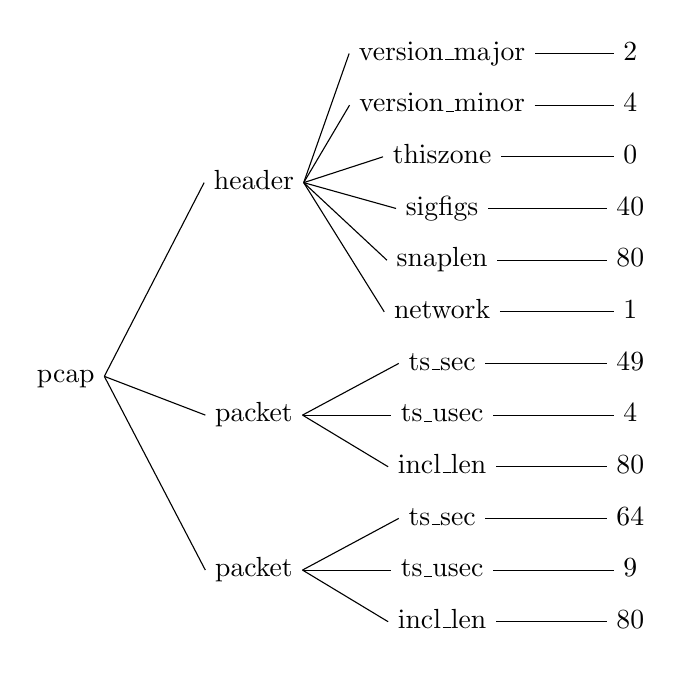
\begin{tikzpicture}[grow=right]
\tikzset{level distance=68pt,sibling distance=0pt}
\tikzset{execute at begin node=\strut}
	\Tree [.pcap 
[.packet [.incl\_len 80 ] [.ts\_usec 9 ] [.ts\_sec 64 ] ]
[.packet [.incl\_len 80 ] [.ts\_usec 4 ] [.ts\_sec 49 ] ]
[.header [.network 1 ] [.snaplen 80 ] [.sigfigs 40 ] [.thiszone 0 ] [.version\_minor 4 ] [.version\_major 2 ] ]
]
\end{tikzpicture}
\end{tabular}
\caption{Example \xml for \texttt{pcap} as Text and Tree}
\label{lst:xmlexample}
\end{listing}
% This listing can probably be made as long as needed to increase the number of pages by adding packets ;)

%### 
\subsubsection{png}
%###
The \textbf{p}ortable \textbf{n}etwork \textbf{g}raphics format is, as its name suggests, a graphics file
format often abbreviated \texttt{png}.
% TODO continue from https://en.wikipedia.org/wiki/Portable_Network_Graphics

% designed for web 
% -> is losslessly compressed (with filter and then DEFLATE)
% -> riddled with CRCs
% => very complex format

% structure: header, chunks (use bytefield), critical, ancillary, public, reserved, copiable
% example chunks: IHDR (introduce color type), PLTE, IDAT, IEND
% conditions on PLTE: essential with 3, optional with 2 and 6, illegal with 0 and 4
% mention schema explosion to model those kinds of dependencies
% mention 3106 LOC of the entire schema


%### 
% \subsubsection{Flac}
%###

%### 
\subsection{Fitness Functions}
%### 
One requirement of this work was to provide \xmlmate with the concept of pluggable fitness functions and 
give several examples that demonstrate the versatility of the approach. Luckily, \evosuite already provides 
a \texttt{FitnessFunction<T extends Chromosome>} generic interface, which can be made use of on multiple 
levels of abstraction. To provide the pluggability on the level of  entire test suites there are implementers of
\texttt{FitnessFunction<XMLTestSuiteChromosome>} and on the level of single test inputs ones of 
\texttt{FitnessFunction<XMLTestChromosome>}. 
Secondary evolution objectives have a very similar type topography; secondary objectives are sometimes useful 
as ``tie breakers'' when a decision between two chromosomes has to be made when both have equal fitness values,
but possess subtle differences that e.g. might lead to slightly more or less favorable crossover behavior in 
the future. The next sections describe some of the new fitness function implementations available with the 
extended and improved \xmlmate.
%### 
\subsubsection{Schema Coverage Fitness Function}
%###
\label{sec:fit:schema}
The very first extension from pure \java branch coverage and exception oriented fitness functions employed 
previously in \xmlmate is the \texttt{Schema Coverage} fitness function. Its goal is to maximize the number 
of schema rules used in the generated inputs. The reasoning behind this is that inputs which exhibit most of 
the features described in the specification should also trigger more functionality in the program under test. 
More concretely the schema coverage fitness value is computed as the average of the folowing three values:
\begin{description}
  \item[element coverage] describes how many element declarations were instantiated in the generated inputs, 
  including substitution group members. A substitution group consists of jointly declared elements, which 
  can take each other's place in the \xml. Additionally, the element coverage can reflect how many branches 
  of choice particles as well as how many of the optional elements are present in the produced files.
  \item[attribute coverage] is, similarly, a measure of how many attribute declarations were utilized, so its 
  value depends on both the optionality of the declarations and the number of generated elements (or more 
  precisely the number of elements carrying the corresponding attribute declarations).
  \item[transition coverage] probably sounds a little out of place, so let me first explain how the concrete 
  values for elements and attributes are generated. One of the most implementation-wise challenging features 
  of the \xsd{} {\small Language} is the \texttt{pattern} facet that describes valid values of an element or 
  attribute by means of a regular expression (that has a different grammar than that of \java, \python or 
  {\small Perl} regular expression languages, which, as an aside, presented another whole technical challenge). 
  In order to be able to provide values conforming to those regular expressions an automaton based representation 
  has been put in place for the types of the elements and attributes. In fact, it worked so well, that there 
  was longer any need in representing any type in a way other than by means of a deterministic finite
  automaton. This means that all types, including \texttt{string}, \texttt{int}, \texttt{short}, \texttt{hexBinary},
  have a corresponding automaton, which is cached in memory for performance reasons. Furthermore, with this representation 
  it is very easy to apply additional facets like restrictions on length or number of fractional digits just by 
  performing automaton based operations like union and intersection. 
  Coming back to the topic of schema coverage, the transitions in these automata are the subject of its 
  transition coverage component which describes how many of the transitions of all the automata are being 
  used in the generated \xml files. This measure is indicative of the overall proportion of covered value space 
  over all type definitions regarded together.
\end{description}

If the element, attribute and transition coverages are designated as $c_e$, $c_a$, and $c_t$ respectively and
are numbers between zero and one, the overall schema coverage fitness value can be computed as $1 -
\frac{c_e+c_a+c_t}{3}$, which makes this a \emph{minimization} fitness function, meaning that the genetic
algorithm of \evosuite will try to get the value as close to zero as possible, which is its default behavior.
    
Contrary to the initial expectations, \improvement{mention in the Evaluation section} the results do not 
necessarily show a strong correlation between high schema coverage and some kinds of code coverage like 
branch or basic block coverage. This can be explained by the fact that it is not the abundance of different 
input values, but rather some specific values themselves, that are responsible for penetrating deeper into a 
program's logic and thus increasing the code coverage.

However, the schema coverage is a good evolution guide for the purpose of creating a diverse starting population
which can then be further evolved with different purposes - be it code coverage of particular program regions, or
other kinds of fitness criteria like closeness to integer overflows and the like.

Furthermore, there is no need in powering up any of the infrastructure involved with usual ways of measuring 
fitness - no system under test, no brokers or converters are needed to compute the schema coverage fitness. 
There is also no need for \texttt{IO} operations, as all \xml tree evaluations are processed in-memory.

%### 
\subsubsection{Basic Block Coverage Fitness Function}
%###
A more or less direct transfer of \evosuite's \texttt{Instruction Count} fitness function is the 
\texttt{Basic Block Coverage} fitness function, which aims to maximize the number of basic blocks 
executed in the program under test. This fitness function makes heavy use of the {\small Intel} \pin
instrumentation framework - in particular its definition of a basic block: a single entrance, 
single exit sequence of instructions in the program under test. However, because \pin is discovering the 
program dynamically as it is executed, its view of basic blocks can be somewhat unconventional. As an 
example consider the code on the left in \cref{lst:bblcode}, which, when compiled for the IA-32 
architecture, will yield instructions approximate to the ones on the 
right\footnote{From \url{https://software.intel.com/sites/landingpage/pintool/docs/67254/Pin/html/\#GRAN}}.
Classically speaking, each \mintinline{nasm}{addl} instruction is its own basic block; however, over the course
of program execution, when the different switch cases are entered, \pin will generate basic blocks, which
contain four instructions as the \texttt{.L7} case is entered, three basic blocks as the \texttt{.L6}
case is entered, and so forth. Furthermore, \pin breaks basic blocks on some other instructions like 
\texttt{cpuid}, \texttt{popf}, and \texttt{REP} prefixed instructions. This leads to a slight divergence 
from the expected values, but for the purposes of representing code coverage this has no negative 
consequences. As a matter of fact, this phenomenon is actually somewhat reminiscent of the LCSAJ
metric\cite{Hennell:1976:PA}, which only increases its value as a fitness score component.
\begin{listing}[h]
\centering
\begin{minipage}[b]{0.49\textwidth}
	\centering
	\begin{ccode*}{linenos=false,frame=bottomline}
	switch(i) {
        case 4: total++;
        case 3: total++;
        case 2: total++;
        case 1: total++;
        case 0:
        default: break;
    	}
\end{ccode*}
	Example C Code
 \end{minipage}
%
 \begin{minipage}[b]{0.49\textwidth}
  \centering
  \begin{minted}[frame=bottomline]{nasm}
.L7:
        addl    $1, -4(%ebp)
.L6:
        addl    $1, -4(%ebp)
.L5:
        addl    $1, -4(%ebp)
.L4:
        addl    $1, -4(%ebp)
\end{minted}
  IA-32 Instructions
 \end{minipage}
 \caption{Example for Basic Block Idiosyncrasies in \pin}
 \label{lst:bblcode}
\end{listing}

The \texttt{Basic Block Coverage} fitness function is the first, but not the only to use the new binary 
backend feature set. Therefore it profits from an abstract fitness function prototype designed specifically 
to work with binary test subjects, which abstracts away and manages the responsibilities of communicating 
with the backend system, be it potential format converters, or the targeted program controlled by test 
drivers and monitored by pintools.
Like all subclasses of this \texttt{BinaryBackendFitnessFunction} the \texttt{Basic Block Coverage} 
fitness function consists of two components: a \java class and a pintool written in \cpp.

The pintool's task is to instrument the targeted binary in such a way, that whenever it executes a 
basic block, which belongs to the image of interest (e.g. \texttt{libpng} - a parameter given at the start),
its address is recorded in a set data structure. When the test driver, which is responsible for running 
the program under test, signals the completion of the processing of the currently evaluated inputs, 
the pintool sends the set as a packet to the \java class in \xmlmate.

It is the purpose of the \java class to interpret the data received from the pintool.
In the case of the \texttt{Basic Block Coverage} fitness function, the data received represents the
set of starting addresses of the basic blocks that were found to be executed in the program under test. 
For each \xml in a test suite an individual set must be maintained in order to be able to profit 
from result caching: when a test suite is modified during the evolution step, not necessarily all
of its tests must have been changed and thus not all tests must be passed to a test driver for reevaluation, 
their previous result can be reused because it is still up-to-date. Virtue of the fact that the pintool 
already builds a set out of the addresses of the executed blocks on its side, the result for a single 
\xml can be stored as an array (\texttt{long[]}) without having to wrap a \texttt{Set} container around it.

However, when it comes to calculating the number of unique basic blocks covered by an 
entire test suite, each time a new set must be created which consists of the union of 
the individual arrays belonging to all \xml files in the suite. At this point the very efficient
\texttt{TLongHashSet} implementation from the \emph{GNU Trove} collections mentioned in \cref{sec:trove} 
is very useful - especially so because it stores the \java primitive values directly instead of \emph{boxing}
them in wrapper objects like the standard \java collections do. This way Trove saves space and is faster.

The actual fitness value of a test suite according to the \texttt{Basic Block Coverage} fitness function 
is the number of unique basic blocks executed by all \xml files in the suite. Due to the dynamic nature 
of instrumentation with \pin it is impossible to know the total number of basic blocks in the program 
under test. One consequence of this is that this fitness function must be a maximization function - meaning
that higher fitness values are considered better, which is somewhat atypical for \evosuite. Even though it has
some degree of support for maximization functions, multiple code defects surfaced during the development that
mostly had to do with hard-coded assumptions about the fitness function always being a minimization function.

%### 
\subsubsection{Basic Block Succession Fitness Function}
%### 
The \texttt{Basic Block Succession} fitness function is an extension of the \texttt{Basic Block Coverage}
fitness function in that it is also heavily based on observing the execution of basic blocks. However, this
extension also considers the order in which the blocks are executed. More specifically, for each basic block
this fitness function aims to maximize the number of unique basic blocks that are executed immediately after.
Put differently, the \texttt{Basic Block Succession} fitness function provides guidance for maximizing the
number of control paths of length two taken by the program under test. According to the
author\footnote{http://lcamtuf.blogspot.de/2014/08/a-bit-more-about-american-fuzzy-lop.html} of the
\texttt{American Fuzzy Lop} smart fuzzing tool\cite{afl} this strategy strikes a good balance between
fitness function complexity and effectiveness, and is very helpful in finding defects.

To accomplish its task, the pintool maintains a map, which contains an address for each basic block that was
observed to be executed as a key. Each key is assigned as value a set of all basic blocks that were executed
immediately after it - be it by fall-through, call, return, or conditional jump. 

The \java part of the \texttt{Basic Block Succession} fitness function receives this map data for each file in
the suite, and collates and merges it into a single basic block successor graph in order to determine the
fitness of the entire suite. The fitness value is then calculated as the number of edges of this graph. 
\improvement[inline]{Add graph example (+merging)}

%### 
\subsubsection{Memory Access}
%###
\label{sec:memcov}
All previously described fitness functions are aimed at increasing a coverage of one sort or another; however,
in the context of using \xmlmate to try and find vulnerabilities in the system under test, this is not
necessarily the most promising approach. In order to be able to find vulnerabilities having to do with
operations such as reading from and writing to memory, such as null pointer dereferences or buffer underflows
or overflows, the first na\"\i{}ve approach is to aim for a maximum number of memory reads and writes at a
maximum of addresses. This is the idea behind the \texttt{Memory Access} fitness function, which like its
cousin \texttt{Basic Block Coverage} fitness function, is a maximization function, with which it also shares
the \texttt{BinaryBackendFitnessFunction} as an ancestor. Once again, this fitness function consists of a
pintool and its complementary \java class. 

The pintool stores memory addresses that were accessed by the program under test in a set, which it sends to
the \java class upon test completion.
The \java class is very similar to that of its cousin fitness function, in fact they share the entirety of
their code.

However, upon consideration of the current use case, the distinction between test suites and tests as
prescribed by \evosuite no longer seems appropriate - what we actually want instead is to evolve a population
of single \xml files in order to find one individual file that triggers faulty behavior. To satisfy this newly
appeared need, the concept of a \emph{singleton population} was introduced.

Using a singleton population is a compromise between \evosuite's need for the presence of test suites to
evolve, and our need for only one set of files to be evolved. When the singleton population is used, the
population size of the genetic algorithm is limited to only one suite and the genetic algorithm itself is
modified accordingly, amongst other things by disabling elitism on the test suite level. Elitism is a
mechanism which ensures that the best individual (the best test suite in \evosuite's case) survives into the
next generation unaltered, so that fitness may never decrease from one generation to the next. Note,
that using elitism does not prevent the best individual from reproducing - its copies may do so freely, and
usually this is what leads to an improvement in fitness. 

With the singleton population in place, there is only one test suite to evolve, which means that the fitness
must now be calculated differently. The fitness of this single suite can no longer reflect the cumulative
result over all the tests, but must rather correspond to the fittest one of them, which, at the end of the
evolution, will be considered the result of the search, or the pinnacle of evolution, if you will.

This routine can be somewhat improved by adding a secondary evolution objective, which considers a
mutation of the test suite as an improvement even if it has the same number of memory accesses in the best
test, yet cumulatively its tests cause more unique memory addresses to be accessed. 

As a technical aside, I want to mention that there were considerations to model the use case of evolving a
set of files as a population of singleton test suites each containing a single file instead of the currently
employed population consisting of one suite. This, however, would have been unfavorable to the parallelization
efforts as per \cref{sec:par} because \evosuite does not allow parallel evaluation of test suites without some
major intrusion in its code base.
%### 
\subsubsection{Division by Zero Fitness Function}
%###
Like the \texttt{Memory Access} fitness function, the \texttt{Division by Zero} fitness function is also
designed to find vulnerabilities in the program under test instead of simply improving test input quality. In
particular, this fitness function aims to uncover a single class of denial of service vulnerabilities -
unhandled arithmetic exceptions that arise from performing division by zero.

When the program under test processes an input file, it usually executes multiple distinct division
instructions, and many of them - multiple times, so there is no simple and obvious way to directly assign a
fitness value to an input file. The first idea is to record all observed instances of division and choose the
smallest absolute value of a divisor as the fitness score. However, such an assignment is not very beneficial
to the diversity of the inputs' gene pool as it makes it converge to smaller files with a minimum number of
executed divisions as long as there is at least one divisor close to zero. Such a constriction opposes the
goal of triggering a division exception as it artificially and unnecessarily limits the number of sites
that are considered for exploration. 

To counteract this effect additional secondary objectives were put in place. The first secondary objective is
the \texttt{MaximizeDivisionsSecondaryObjective} and its goal is to enlarge the number of sites in the
program under test that are being explored by the search process by increasing the number of division
instructions covered by a suite. Using only this single secondary objective, however, leads to individuals
simply growing in size over the course of evolution, while keeping at least one close-to-zero divisor. While
this is beneficial to the diversity of the suites, it causes an unwelcome strain on the performance, which
is why another secondary - or rather a tertiary - objective has been added - the
\texttt{MinimizeCumulativeZeroDistanceSecondaryObjective}. The goal of this objective is to prevent an
uncontrolled growth and ensure overall improvement of quality of the individuals by keeping the cumulative
divisor distance to zero as small as possible.

At runtime the pintool component of the \texttt{Division by Zero} fitness function intercepts all invocations
of the \texttt{DIV} and \texttt{IDIV} x86 instructions and records the divisor value in a list, which is
associated with the address of the instruction in question by means of a map container. When the execution of
the system under test has ended, for each division instruction the pintool keeps only the divisor with the
smallest zero distance when it packages the message to be sent out to its \java fitness function counterpart.
There is a reason behind selecting the best divisor only after the main runtime instead of doing it on-the-fly,
even though it wastes some memory space for storing all observed divisors. This is an instance of the classical
runtime vs memory requirement trade off: by having injected code simply append any new value to a list
instead of doing comparisons to decide whether to keep or reject the new value, the code is simple enough to
be inlined and thus performs considerably faster; and with main memory being available in abundance on  modern
computers and execution speed being the most limiting factor, it seems like a good trade off to make.

Because the \texttt{Division by Zero} fitness function is meant to be used for vulnerability scanning, it is
exclusively compatible with the singleton population evolution mode introduced in \cref{sec:memcov}. The \java
component of this fitness function keeps a record of all executed division instructions alongside the absolute
value of their divisor closest to zero for each file in a suite. The overall fitness score of the entire suite
is then determined by finding the minimal divisor distance over all division instructions over all files in
the suite.

As previously suggested, this fitness function currently only supports integer based division instructions
because \pin imposes a limitation on retrieving floating point values from
registers\footnote{\url{https://software.intel.com/sites/landingpage/pintool/docs/67254/Pin/html/index.html\#FP}}.
Working around this and adding support for \texttt{SIMD} instructions are some planned future improvements.

An intuition is that it is unusual for valid well formed inputs to cause divisions by zero in the program under
test. It is therefore recommended to use the local search feature described in \cref{sec:local}, which is
capable of producing values beyond the range of validity, in order to increase the chances of actually
triggering arithmetic exceptions.

%### 
%\subsubsection{Context Switches Fitness Function}
%### 
% TODO mention in future work section
 
%### 
\subsubsection{Integer Overflow Fitness Function}
%### 
Continuing in the vein of fitness functions specialized in narrow categories of vulnerabilities, the next
fitness function is the \texttt{Integer Overflow Fitness Function}. Just as the name suggests, its aim is to
guide the evolution of inputs towards causing an unhandled integer overflow. Integer overflows are often
suitable as vessels for denial of service attacks as well as access control attacks, and therefore of
critical severity. 

In order to achieve its goal the \texttt{Integer Overflow} fitness function\ldots
\change[inline]{complete}
% method - multiplications (and additions)
% need for local search
% singleton population
% standard secondary objectives?

%### 
\subsubsection{Buffer Overflow Fitness Function}
%###
\change[inline]{complete}
% motivation
% method and relation to memory access fitness function
% mention implementation difficulties:
% 	multithreading issues -> interleaving -> solution additionally map by thread_id / use thread local storage
% 	however point_after is unreliable (https://software.intel.com/sites/landingpage/pintool/docs/67254/Pin/html/#Invocation) and so a replacement must be used
% singleton population
% secondary objectives
% local search
\section{Evaluation}
\label{sec:evaluation}
\subsection{Subjects}
\tocless\subsubsection{libxml2}
\tocless\subsubsection{libpng}
% mention generating only 2x2 pixels
\tocless\subsubsection{libpcap}
%\subsubsection{libflac}
\subsection{Results}
\subsection{Threats to Validity}
\section{Conclusion}
\label{sec:conclusion}
% xmlmate is a good defect search tool with extensions presented here
% list extensions: support for binaries, pluggable fitfuncs, additional formats, schema violations
% equipped with these extensions xmlmate yielded good results in identifying defects
% its efficiency and effectiveness are justified by it finding known vulns a lot of times over
% its practical use is strengthened by it finding unknown bugs even when not specifically targeting 
% overall xmlmate shows potential
% quality of results (fitness scores and crashes) depends on quality of test drivers and schema and converters
% 		=> future work items
\section{Future Work}
\label{sec:future}
The presented approach paves the way for many more useful improvements and extensions on numerous facets and
aspects of \xmlmate. This section gives a brief overview of some of the most interesting future work items.
\begin{itemize}
\item[]One particularly large work item is completely rewriting the genetic algorithm of \xmlmate from scratch
aiming for better parallelization support from the beginning. At the time of writing it is estimated that this
goal is best achieved by making heavy use of many of the features that the {\small
Scala}\cite{scala-overview-tech-report} programming language has to offer, as well as utilizing the {\small
Akka} actor-based message-driven concurrency framework\cite{Wyatt:2013:AC:2663429} to make \xmlmate fully
concurrent and distributed.
\item[]To make better use of the available computational resources, the genetic algorithm at the heart of
\xmlmate can profit from the addition of meta-heuristics that would govern the number of instances of certain
subprocesses like format converters or worker nodes during runtime based on the proportion of their
respective load on the system.
\item[]Delving deeper into the use case of finding vulnerabilities, it might be wise to further investigate
the mechanism responsible for generating aberrant and unexpected input values and extend it to work not only
with integer and floating point types, but other types and even structures permissible in \xml as well.
\item[]Since \xmlmate provides an interface for pluggable fitness functions, it is only natural to want to try
out more of them. Some next candidates would be the branch coverage fitness function as implemented in
\evosuite in the context of generating test suites, and for program resilience testing purposes a fitness
function that aims to maximize the number of context switches in a concurrent program seems interesting for
finding multi-threading related issues such as deadlocks, livelocks, starvation and the like.
\item[]For future fitness functions that use program performance values in the computation of their
fitness score it is possible to significantly increase efficiency by making use of hardware performance
counters, which are provided by modern hardware and can be directly accessed in most operating systems by
means of special APIs like the one provided by the {\small PAPI}\cite{Mucci99papi:a} library. Note that
this would impose a limitation on the concurrent use of \xmlmate on a single machine; however, this limitation
can probably be solved by using virtualization techniques like {\small Docker}\cite{docker} and {\small
Vagrant}\cite{vagrant} - especially since \xmlmate is now a distributed system capable of running across
multiple heterogeneous nodes.
\item[]If \xmlmate is going to be used in truly distributed systems, it is probably a good idea to replace
the currently employed \msgpack message serialization and deserialization engine by another, more efficient and
sophisticated library. When real network traffic is involved, it seems like a good idea to minimize the amount
of traffic that has to pass through the network, and having a library with a streaming interface that also
allows to deserialize messages before they have reached their destination completely is certainly also of
good use as well. Some candidate replacements can be found in \cref{sec:msgpack}.
\item[]With more fitness functions come more test subjects that can be explored. For formats, for which the
corresponding schemas and converters already exist in the current version, such applications as \emph{tcpdump}
and \emph{tshark} for the \pcap format and a whole
lot\footnote{\url{http://www.libpng.org/pub/png/pngapcv.html}} of programs for {\small png} are available.
\item[]Adding test subjects that process other file formats requires adding new schemas and converters that
support them. Some envisioned targets are \emph{libjpeg}, \emph{giflib} and \emph{libflac} libraries for
processing image, animation and sound files, respectively.
\item[]In terms of usability and convenience \xmlmate could profit from minimizing the files responsible for
revealing a defect in the application under test using delta debugging\cite{zeller2002simplifying} to make it
easier for the user to find the actual cause of the failure in question.
\item[]Ending on another big topic, seeing as \xmlmate has its origins in the \java world, it could be extended
to support testing of \java applications that use native code by performing instrumentation on both \java
byte code and the native binary code.
\end{itemize}

% add electric fence? (maybe to the same item as PAPI)
% add multiplatform support? (windows?)
% add reliability protocol? (on top of zmq)
\newpage
\section*{References}
\renewcommand\refname{}
\addcontentsline{toc}{section}{References}
\bibliographystyle{plain}
\bibliography{sources}
\end{document}
